\subsection{Data Collection}
\label{sec:data_methods}

\subsubsection{Workspace Coordinate Frame Definition}
The workplace has a coordinate frame defined by three point markings on the green acrylic sheet at three corners (shown in Figure \ref{fig:workspace}). During regular operation of the robot, all readings from the AURORA system are transformed to be represented in the workspace coordinate frame (sometimes referred to as the "robot frame"). A method is used to calibrate the reference frame between each session on the robot. A total of 30 AURORA measurements are taken at each of the three points. The average position of the points is found by a simple mean over the 30 readings. The origin of the workspace is taken to be the location of the first point, $O_1$. The workspace axes are defined as follows: 

\begin{align*}
    \hat{x} &= \frac{O_3 - O_1}{||O_3 - O_1||} \\
    \tilde{y} &= \frac{O_2 - O_1}{||O_3 - O_1||} \\
    \hat{z} &= \hat{x}\times\tilde{y} \\
    \hat{y} &= \hat{z}\times\hat{x}
\end{align*}

\begin{figure}[h]
    \centering
    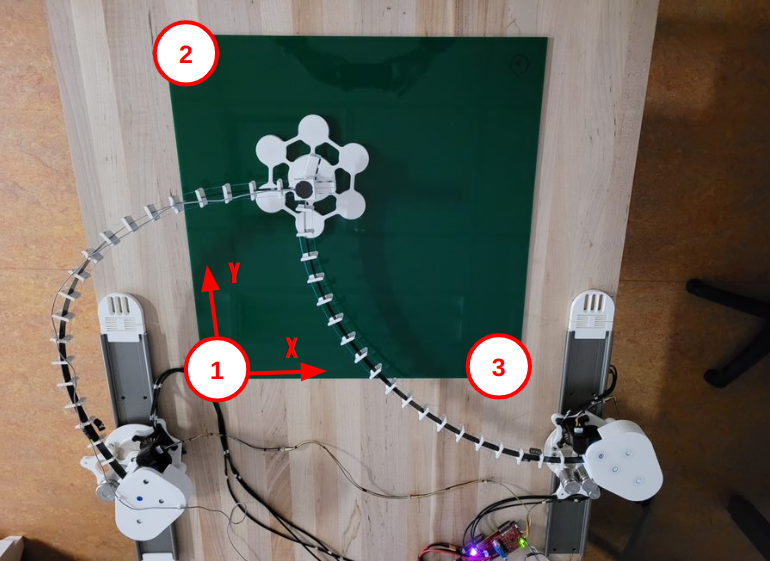
\includegraphics[width=0.8\textwidth]{images/workspace.png}
    \caption{Robot workspace coordinate frame diagram}
    \label{fig:workspace}
\end{figure}


\subsubsection{Data Schema}
Data is collected from all parts of the system at various rates as described in Table \ref{tab:data_schema}. All data during operation is saved to log files with unique names that can later be loaded into a dataloader object. 

\begin{table}[h]
    \centering   
    \caption{Robot data collection schema}
    \begin{tabular}{p{0.5\linewidth} | p{0.15\linewidth} | p{0.2\linewidth}}
        \textbf{Data Type} & \textbf{Unit} & \textbf{Frequency in Hz} \\
        \hline
        \multicolumn{3}{c}{Motor Controller} \\
        \hline
        Current command & A & 100 \\
        Current draw & A & 100 \\
        Motor position set point & rad & 100 \\
        Motor position & rad & 100 \\
        Motor angular velocity set point & rad/s & 100 \\
        Motor angular velocity & rad/s & 100 \\
        Controller type & N/A & 100 \\
        Recording timestamp & s & 100 \\
        \hline
        \multicolumn{3}{c}{AURORA System} \\
        \hline
        End effector position (AURORA frame) & m & 5 \\
        End effector orientation (AURORA frame) & m & 5 \\
        End effector position (robot frame) & m & 5 \\
        Recording timestamp & s & 5 \\
        \hline
        \multicolumn{3}{c}{Robot Commander} \\
        \hline
        Sample termination cause & From table \ref{tab:termination_types} & On termination \\
        Commander state & From table \ref{tab:controller_states} & 5 \\
        Recording timestamp & s & 5 \\
        \hline
    \end{tabular}
    \label{tab:data_schema}
\end{table}


\subsubsection{Collection Method}
\paragraph{The robot controller} used for data collection is the prismatic assumption PID baseline controller from Equation \eqref{eq:pid/complete}. It was selected because of its good relative performance on a number of metrics discussed in Section \ref{sec:baseline_comparison}. Data was only collected using this single baseline due to project timing limitations. As such, the data collected only contains robot states that are accessible using this controller, which has the potential to instill bias into the dataset. 

\paragraph{The sampling method} used for deciding which paths to move the robot over is a random sampling over a uniform distribution. Sample goal points are drawn inside a \SI{15}{cm} radius of the end effector position at the start of the sample and outside a \SI{5}{cm} radius of that same position. An upper bound of \SI{15}{cm} was selected as much above that would result in harsh robot movements that caused damage to the robot. A lower bound of \SI{5}{cm} was selected as much below that would result in motor set points that result in an applied motor torque that is too low to overcome the static friction of the end effector in some positions in the workspace. 

A more complex path sampler was explored using randomized path generation while ensuring joint actuation smoothness, but was ultimately removed as it did not satisfy the workstation's real time runtime constraints. More information on this method is presented in Appendix \ref{app:path_planner}. 


\subsubsection{Termination Cases}
\paragraph{Non-critical failures} occur when for some reason the robot is not able to find a way to withing a \SI{2}{cm} radius of the sampled goal point. A number of reasons can cause this, including lost AURORA measurements or a stalled end effector. The robot can recovery without user intervention from non-critical failure cases and the data from them is complete and usable. 

\paragraph{Critical failures} occur when the robot failed in a way that could result in corrupted data. This happens when a portion of the code crashes or the robot loses power, typically by the user hitting the emergency stop. In critical failure cases the user must reset the system manually and delete the affected data logs. 

\paragraph{Successful samples} occur when the robot successfully arrives at the sampled goal point without triggering any of the failure cases. A full description of all termination causes is provided in Table \ref{tab:termination_types}. 

\begin{table}[h]
    \centering   
    \caption{Robot sample termination types}
    \begin{tabular}{p{0.3\linewidth} | p{0.6\linewidth}}
        \textbf{Termination Type} & \textbf{Description} \\
        \hline
        Success & The robot successfully reached the target point \\\hline
        Stalled & The robot's end effector velocity was below \SI{0.001}{m/s} for more than \SI{5}{s} \\\hline
        Aurora lost & At least 3 consecutive AURORA measurements were errors, typically caused by the end effector leaving the workspace \\\hline
        Recovery & The robot underwent recovery behaviour where AURORA readings are not necessarily available \\\hline
        Mode switch & The robot operator manually switched the robot into a different mode \\\hline
        User terminated & The user shut down the system using the control interface \\\hline
        Tracking finished & A reference trajectory was completed \\\hline
        Error & An error is raised during the trial. This results from a crashed thread, or a failed recovery attempt \\\hline

    \end{tabular}
    \label{tab:termination_types}
\end{table}